\item \points{2f} \textbf{Coding problem.}

Using the validation set, estimate the constant $\alpha$ by averaging your
classifier's predictions over all labeled examples in the validation set:\footnote{There is a reason to use the validation set, instead of the training set, to estimate the $\alpha$. However, for the purpose of this question, we sweep the subtlety here under the rug, and you don't need to understand the difference between the two for this question. } 
%
\begin{equation*}
  \alpha \approx \frac{1}{\mid V_{+} \mid}\sum_{x^{(i)}\in V_{+}} h(x^{(i)}).
\end{equation*}
%
Add code in \texttt{src/submission.py} to rescale your
 predictions $h(y^{(i)}=1\mid x^{(i)})$ of the classifier that is obtained from part b,  using the equation~\eqref{eqn:3} obtained in part (d) and using the estimated value for $\alpha$. 
More specifically implement the |find_alpha_and_plot_correction| function.

 The output plot should look similar to the following (no plot submission is required):
 \begin{figure}[H]
   \centering
   \vspace{2mm}
   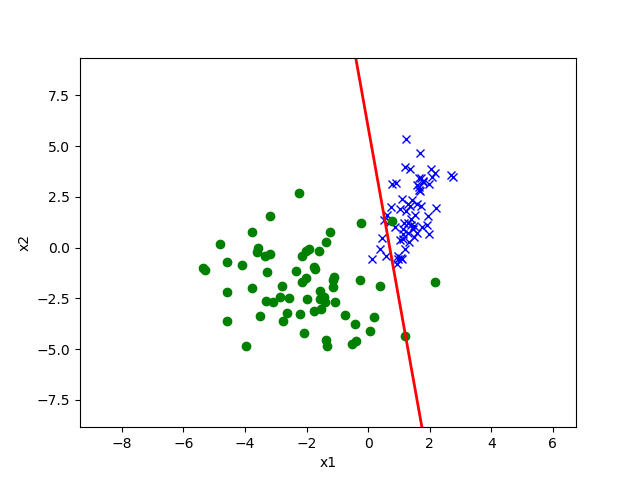
\includegraphics[width=0.5\linewidth]{02-posonly/posonly_adjusted_pred.png}
     \caption{Separating hyperplane for logistic regression on training set using using corrected alpha value from validation set (Note: This is for reference only.  You are not required to submit a plot.)}
 \end{figure}

